%
%\documentclass[twocolumn,showpacs,preprintnumbers,amsmath,amssymb, floatfix]{revtex4}
\documentclass[aps,prb,preprint,preprintnumbers,amsmath,amssymb,floatfix,superscriptaddress]{revtex4}
%\documentclass[aps,prb,twocolumn,preprintnumbers,amsmath,amssymb,floatfix]{revtex4}

% Some other (several out of many) possibilities
%\documentclass[preprint,aps]{revtex4}
%\documentclass[preprint,aps,draft]{revtex4}
%\documentclass[prb]{revtex4}% Physical Review B

\usepackage{graphicx}% Include figure files
\usepackage{dcolumn}% Align table columns on decimal point
\usepackage{bm}% bold math
\usepackage{verbatim}
\usepackage{array}
\usepackage{hyperref}
\usepackage{epstopdf,subfigure}

\usepackage{natbib}

\newcolumntype{x}[1]{%
>{\centering\hspace{0pt}}p{#1}}%

%Definition of new commands
\newcommand{\be} {\begin{eqnarray}}
\newcommand{\ee} {\end{eqnarray}}
\newcommand{\f}[2]{\ensuremath{\frac{\displaystyle{#1}}{\displaystyle{#2}}}}
\newcommand{\lr}[1]{\langle{#1}\rangle}

\begin{document}
\title{A Review of Models for Predicting the Thermal Conductivities of Bulk Materials and the Thermal Boundary Resistances of Interfaces}

\author{S. C. Huberman}
\affiliation{Department of Mechanical \& Industrial Engineering, University of Toronto, 
Toronto, Ontario M5S 3G8, Canada}

\date{\today}% It is always \today, today,
             %  but any date may be explicitly specified

\vspace{14mm}    
\begin{abstract}
A review of the methods for predicting the thermal conductivity of a material from atomistic approaches is presented. Beginning with the relevant theory, three methods are discussed; the Green-Kubo (GK) method, the Direct Method (DM) and the Spectral Energy Density through Normal Mode Decomposition (SED-NMD) approach. The second part of this report reviews the theory and models of thermal boundary resistance. The final section outlines the current attempt to investigate phonon properties near an interface.


\end{abstract}
\maketitle

\section*{Introduction}
The classical problem of predicting material properties remains to a challenge to the present day. However, the arsenal of tools has become increasingly powerful with the steady advance of computational perfomance in accordance with Moore's Law. Indeed, computational techniques like Density Functional Theory (DFT), Quantum Monte Carlo (QMC), and classical Molecular Dynamics (MD) have transitioned to the realm of the desktop PC (albeit for simple systems).

By directly evaluating the equations of motions for the system's particles (Newton's 2nd law for atoms in classical MD, Schrodinger's equation for electrons in DFT or QMC), macroscopic properties like electrical or thermal conductivity can be abstracted through the statistical behaviour of the particles' phase coordinates (e.i.: position and momentum). Several of such abstractions are reviewed here.    

\subsection*{Fluctuation-Dissipation Theorem}

The Fluctuation-Dissipation Theorem (FDT), first stated by Harry Nyquist, was later reformulated by Ryogo Kubo to relate transport coefficients to equilibrium time correlation functions \cite{JPSJ.12.570}. What follows is an outline of the logic of Kubo's generalization of the FDT using Helfand's approach as reviewd by McQuarrie\cite{mcquarrie}. Beginning with the diffusion equation
%
\begin{equation}
\frac{\partial G(\pmb{r},t)}{\partial t}= D \nabla ^2G(\pmb{r},t).
\end{equation}
%
Here, $G(\pmb{r},t)$ is the fraction of particles in phase coordinates about $d\pmb{r}$ at $\pmb{r}$ at time $t$ given that they were located at $\pmb{r}(0)$ at $t=0$
%
\begin{equation}
G(\pmb{r},t)= \frac{1}{N}\left<\sum_{j=1}^N\delta(\pmb{r}-[\pmb{r}_j(t)-\pmb{r}_j(0)])\right>.
\end{equation}
%
At this point, it is insightful to take the Fourier transform of $G(\pmb{r},t)$ as it provides the form of the time correlation function, $<A^*(t)A(0)>$
%
\begin{equation}
F(\pmb{\kappa},t)=\int_{-\infty}^{\infty}G(\pmb{r},t)e^{-i\pmb{\kappa}\cdot\pmb{r}}d\pmb{r}=\frac{1}{N}\left<\sum_{j=1}^Ne^{i\pmb{\kappa}\cdot\pmb{r}_j(t)}e^{-i\pmb{\kappa}\cdot\pmb{r}_j(0)}\right>.
\end{equation}
%
Recalling the basic kinematic relations in the most general forms
%
\begin{equation}
\pmb{r}(t)-\pmb{r}(0)=\int_0^t \pmb{v}(t')dt'
\end{equation}
\begin{equation}
[\pmb{r}(t)-\pmb{r}(0)]^2=\int_0^t \int_0^t \pmb{v}(t')\cdot\pmb{v}(t'')dt'dt''.
\end{equation}
%
The usefulness of Equation 5 becomes clear upon taking the ensemble average thus giving the average behaviour of all possible functions of the phase coordinates $\pmb{r},\pmb{v}$
%
\begin{equation}
<[\pmb{r}(t)-\pmb{r}(0)]^2>=\int_0^t \int_0^t <\pmb{v}(t')\cdot\pmb{v}(t'')>dt'dt''.
\end{equation}
%
Since the ensemble is a stationary process (e.i.: independent of the definition of the origin of time) and the classical equations of motion are time-symmetric
%
\begin{equation}
<\pmb{v}(t')\cdot\pmb{v}(t'')>=<\pmb{v}(t'-t'')\cdot\pmb{v}(0)>=<\pmb{v}(t''-t')\cdot\pmb{v}(0)>.
\end{equation}
%
From the initial solution to the diffusion equation $<[\pmb{r}(t)-\pmb{r}(0)]^2>=6Dt$, substituting $\tau=t''-t'$ and performing the first integration
%
\begin{equation}
6Dt=2t\int_0^t\left(1-\frac{\tau}{t}\right)<\pmb{v}(\tau)\cdot\pmb{v}(0)>d\tau.
\end{equation}
%
Assuming that the time correlation function decays to zero long before $t$, the final form can be taken
%
\begin{equation}
D=\frac{1}{3}\int_0^{\infty}<\pmb{v}(\tau)\cdot\pmb{v}(0)>d\tau.
\end{equation}
%
and thus arriving at an expression for the diffusion coefficient in terms of the equilibrium time correlation function for velocity. Kubo generalized this result by expressing the linear response of a system from small perturbations in terms of its fluctuations about equilibrium.

\subsection*{Wiener-Khintchine Theorem}

As is happens, the usefulness of the (time) correlation functions extends well beyond the FDT. An simple example is the Wiener-Khintchine Theorem (WKT), which relates the correlation function of a continuous stationary random process to its' spectral density. The correlation function of a time-dependent quantity (i.e: position, velocity, etc.) is defined as the average behaviour in time of said quantity \cite{mcquarrie}
%
\begin{equation}
C(t)=\lim_{T->\infty}\frac{1}{2T}\int_{-T}^{T}x(t+t')x(t')dt'.
\end{equation}
%
From the ergodic hypothesis, which states that the statistical properties of a large number of observations at $N$ arbitrary times from a single system are equivalent to the statistical properties of $N$ obervations made from $N$ equivalent systems made at the same time, the correlation function can be rewritten as an ensemble average
%
\begin{equation}
C(t)=<x(t+t')x(t')>.
\end{equation}
%
Let's define $X(\omega)$ as the Fourier Transform of $x(t)$
%
\begin{equation}
X(\omega)=\int_{-\infty}^{\infty}x(t)e^{-i\omega t}dt.
\end{equation}
%
Recalling Parseval's theorem, which states that the integral of the square of a function is equal to the integral of the square of it's transform
%
\begin{equation}
\int_{-\infty}^{\infty}x^2(t)dt=\frac{1}{2\pi}\int_{-\infty}^{\infty}|X(\omega)|^2d\omega.
\end{equation}
%
Noting that $\int_{-\infty}^{\infty}x^2(t)dt=<x^2>$, let $S(\omega)$ be the spectral density of $x(t)$
%
\begin{equation}
S(\omega)=\lim_{T->\infty}\frac{1}{2T}|X(\omega)|^2.
\end{equation}
%
From the Parseval's theorem equality
%
\begin{equation}
<x^2>=\frac{1}{2\pi}\int_{-\infty}^{\infty}|X(\omega)|^2d\omega.
\end{equation}
%
To offer an intuitive interpretation of this result, take $x(t)$ to be an electric current and $<x^2>$ to be the average power dissipated as the current passes through a circuit. In this case, $X(\omega)d\omega$ will be the average power dissipated with frequencies between $\omega$ and $\omega+d\omega$. The WKT extends this result to the correlation function
%
\begin{equation}
C(t)=\frac{1}{2\pi}\int_{-\infty}^{\infty}C(\omega)e^{i\omega t}d\omega
\end{equation}
%
\begin{equation}
C(\omega)=\int_{-\infty}^{\infty}C(t)e^{-i\omega t}dt.
\end{equation}
%
Taking an example from Dove \cite{dove}, let $x$ have only two equally probably values of $\pm 1$ with the probability of $x$ changing it's value during $dt$ of $dt/\tau$, where $\tau$ represents the average time between value changes. The correlation function is
%
\begin{equation}
C(t)=e^{\frac{-|t|}{\tau}}.
\end{equation}
%
The spectral density is then
\begin{equation}
C(\omega)=\int_{-\infty}^{\infty}e^{\frac{-|t|}{\tau}}e^{-i\omega t}dt=\frac{2\tau}{1+(\omega \tau )^2}
\end{equation}
which is a Lorentzian centred about zero frequency and $\tau$ is the half width at half-maximum (HWHM).
\section*{The Green-Kubo Method}

The GK relation for thermal conductivity falls out of the fluctuation-dissipation theorem and the assumptions made therein, namely that the perturbations to the system's Hamiltonian are small and that the stochastic processes are Markoffian \cite{green:398}. Thus the thermal conductivity can be related to the fluctuations of the heat current vector, $\pmb{S}$, over long periods
%
\begin{equation}
k=\frac{1}{k_B V T^2}\int_0^{\infty}\frac{<\pmb{S}(t)\cdot\pmb{S}(0)>}{3}dt.
\end{equation}
%
The heat current vector is given by 
%
\begin{equation}
\pmb{S}=\frac{d}{dt}\sum_i\pmb{r}_iE_i
\end{equation}
%
where $E_i$ is the energy of particle $i$ at position $\pmb{r}_i$. $<\pmb{S}(t)\cdot\pmb{S}(0)>$ is referred to as the heat current autocorrelation function (HCACF). For pairwise potentials, the heat current vector is
%
\begin{equation}
\pmb{S}=\sum_ie_i\pmb{v}_i+\frac{1}{2}\sum_{i,j}(\pmb{F}_{ij}\cdot\pmb{v}_{i})\pmb{r}_{ij}.
\end{equation}
%
Equations 21 and 22 can be easily added to a MD code since the quantities with which $\pmb{S}$ is calculated, typically, are tracked for every time step. McGaughey examined the time dependence of the HCACF and noted a two stage behaviour for crystals: a rapid initial decay corresponding to the damping of the fluctuations and a slow secondary oscillatory decay, which is believed to be associated with the periodic boundary conditions of the simulation. These oscillations decreased as the simulation size was increased \cite{mcgaugheythesis}.

For cases where the HCACF converges well, the thermal conductivity can be found by numerically integrating over a suitable range. Li et al. \cite{Li1998139} use two methods to determine objectively determine the definition of suitable range. One method is simply to evaluate the integral to the point where the HCACF first becomes negative, known as the first dip method. For cases where the HCACF remains positive, an exponential fit is used to determine the contribution of the tail.

In the case of amorphous materials, the HCACF does not converge prior to becoming negative, thus the first dip or exponential fit methods cannot be used and \textit{a priori} knowledge of the functional form of the HCACF is required in order to complete the integration and predict thermal conductivity.

\section*{The Direct Method}

Unlike the GK method, the direct method uses a non-equilibrium steady-state approach to determine thermal conductivity. A one-dimension heat flux is generated through the simulation, typically by keeping the boundaries of the simulation at fixed, but different, temperatures, such that the boundaries behave like a hot and cold thermodynamic bath. From Fourier's law, the thermal conductivity can be predicted once the heat flux has converged
%
\begin{equation}
k=-\frac{q_x}{dT/dx}.
\end{equation}
%
Equivalently, a heat flux can be imposed and the corresponding temperature difference calculated. Generally, both set-ups are used, but the time to convergence of the heat flux vector is orders of magnitude greater than that of the temperature difference.

The applicability of direct method is questionable in situations where the temperature profile is not linear. Such is the case for nanoscale systems with a temperature difference on the order of 10K \cite{mcgaugheythesis}.

\section*{SED-NMD}

In order to overcome the limitations of the DM and GK method, scientists have turned to the Boltzmann Transport Equation (BTE). Although analytically intractable, there exists a multitude of computational solutions for the BTE. Under the relaxation time approximation and from Fourier's law, the thermal conductivity can be expressed in terms of contributions over all possible phonon modes \cite{sellan_CP}
%
\begin{equation}
	k_{z}= \sum_\nu\sum_\kappa c_{ph}(\pmb{\kappa},\nu)v^2_{g,z}(\pmb{\kappa}, \nu)\tau_{p-p}(\pmb{\kappa}, \nu).
\end{equation}
%
Here $c_{ph}(\pmb{\kappa},\nu)$ is the volumetric specific heat from the classical thermodynamic definition
%
\begin{equation}
c_{ph}(\pmb{\kappa},\nu)=\frac{\partial E}{V\partial T}=\frac{\hbar\omega(\pmb{\kappa},\nu)}{V}\frac{\partial f^{BE}(\pmb{\kappa}, \nu)}{\partial T}	
\end{equation}
%
and
\begin{equation}
v_{g,z}(\pmb{\kappa}, \nu)=\frac{\partial \omega(\pmb{\kappa},\nu)}{\partial \pmb{\kappa}}
\end{equation}
is the group velocity in the $z$ direction which can readily obtained from harmonic lattice dynamics. The final and missing piece is the lifetime of a given mode $\tau_{p-p}(\pmb{\kappa}, \nu)$ which arises as a result of the intrinsic anharmonicity of the interatomic potential and is responsible for finite thermal conductivity and thermal expansion. In the past decade, significant progress has been to computationally predict this property. Broido et al. used Density Functional Perturbation Theory (DFPT) \cite{Broido1} while Esfarjani et al. used a DFT-MD approach \cite{PhysRevB.84.085204}. The method proposed by Larkin \cite{larkin} involves the calculation of the spectral energy density of the normal modes (SED-NMD). Although this approach relies on the empirical potentials of classical MD, the complete anharmonicity is considered, an advantage it posesses over other methods, like DFPT which truncate terms beyond the third order derivatives. SED-NMD is an algorithm that combines time-dependent information from molecular dynamics and the harmonic solutions from lattice dynamics to infer the phonon lifetimes From harmonic lattice dynamics, the displacement of atom $j$ in unit cell $l$ at time $t$ is represented as a superposition of waves of wavevector $\pmb{\kappa}$ with amplitude $\pmb{U}(j,\pmb{\kappa},\nu)$
\begin{equation}
\pmb{u}(jl,t)=\sum_{\pmb{\kappa},\nu}\pmb{U}(j,\pmb{\kappa},\nu)exp(i[\pmb{\kappa}\cdot\pmb{r}(jl)-\omega(\pmb{\kappa},\nu)t])=\frac{1}{\sqrt{Nm_j}}\sum_{\pmb{\kappa},\nu}\pmb{e}(j,\pmb{\kappa},\nu)exp(i\pmb{\kappa}\cdot\pmb{r}(jl))Q(\pmb{\kappa},\nu)
\end{equation}
with $Q(\pmb{\kappa},\nu)$ being the normal code coordinate and $\pmb{e}(j,\pmb{\kappa},\nu)$ being the eigenvector determined from the eigenvalue problem $\omega^2(\pmb{\kappa},\nu) e(\pmb{\kappa},\nu)=D(\pmb{\kappa})e(\pmb{\kappa},\nu)$. To rearrange for the normal mode, mulitply Equation 27 with $\pmb{e}^*(j,\pmb{\kappa},\nu)$ to take advantage of the orthogonality of the eigenvectors
\begin{equation}
\pmb{e}^*(j,\pmb{\kappa},\nu)\pmb{u}(jl,t)=\frac{1}{\sqrt{Nm_j}}exp(i\pmb{\kappa}\cdot\pmb{r}(jl))Q(\pmb{\kappa},\nu).
\end{equation}
Taking the Fourier Transform
\begin{equation}
\int_{-\infty}^{\infty}\pmb{e}^*(j,\pmb{\kappa},\nu)\pmb{u}(jl,t)exp(-i\pmb{\kappa}\cdot\pmb{r}(jl))d\pmb{r}=\frac{1}{\sqrt{Nm_j}}\int_{-\infty}^{\infty}Q(\pmb{\kappa},\nu)d\pmb{r}
\end{equation}
and noting that $\int_{-\infty}^{\infty}d\pmb{r}=N$, gives the expression for the normal coordinate
\begin{equation}
Q(\pmb{\kappa},\nu,t)=\frac{1}{\sqrt{N}}\sum_{jl}\sqrt{m_j}exp(-i\pmb{\kappa}\cdot\pmb{r}(jl))\pmb{e}^*(j,\pmb{\kappa},\nu)\cdot\pmb{u}(jl,t).
\end{equation}
The time derivative of the normal mode is
\begin{equation}
\dot{Q}(\pmb{\kappa},\nu,t)=\frac{1}{\sqrt{N}}\sum_{jl}\sqrt{m_j}exp(-i\pmb{\kappa}\cdot\pmb{r}(jl))\pmb{e}^*(j,\pmb{\kappa},\nu)\cdot\dot{\pmb{u}}(jl,t).
\end{equation}
The harmonic Hamiltonian of the lattice can thus be represented in terms of normal modes
\begin{equation}
H=\frac{1}{2}\sum_{\pmb{\kappa},\nu}\dot{Q}(\pmb{\kappa},\nu)\dot{Q}^*(\pmb{\kappa},\nu)+\frac{1}{2}\sum_{\pmb{\kappa},\nu}\omega^2(\pmb{\kappa},\nu)Q(\pmb{\kappa},\nu)Q^*(\pmb{\kappa},\nu).
\end{equation}
The first term on the right hand side corresponds to the kinetic energy while second term corresponds to the potential energy. By taking a series of velocity samples from an equilibrium MD simulation of time interval (in signal processing terminology, this is known as lag which is symbolically represented here by $t$) an order of magnitude shorter than inverse of the highest frequency present in the system (known from solutions to the aforementioned eigenvalue problem) and using Equation 31 to project the sampled velocities onto the eigenvectors, the autocorrelation of the normal modes can calculated by
\begin{equation}
C(\pmb{\kappa},\nu,t)=\lim_{T->\infty}\frac{1}{T}\int_{0}^{T}Q(\pmb{\kappa},\nu,t+t')Q(\pmb{\kappa},\nu,t')dt'.
\end{equation}
The spectral energy density, from the WKT, is thus
\begin{equation}
C(\pmb{\kappa},\nu,\omega)=\int_{-\infty}^{\infty}C(\pmb{\kappa},\nu,t)e^{-i\omega t}dt
\end{equation}
which, like Equation 19, is a Lorentzian centered at $\omega_0(\pmb{\kappa},\nu)$
\begin{equation}
C(\pmb{\kappa},\nu,\omega)=\frac{C_0(\pmb{\kappa},\nu)}{2}\frac{\Gamma(\pmb{\kappa},\nu)/\pi}{(\omega_0(\pmb{\kappa},\nu)-\omega)^2+\Gamma(\pmb{\kappa},\nu)}.
\end{equation}
The HWHM is related by anharmonic lattice dynamic theory \cite{PhysRev.128.2589} to phonon lifetime by
\begin{equation}
\tau_{p-p}(\pmb{\kappa}, \nu)=\frac{1}{2\Gamma(\pmb{\kappa},\nu)}
\end{equation}
The interpretation of this relation can be understood through a qualitative argument from time-dependent perturbation theory (TDPT). Using TDPT, the anharmonic terms in the complete Hamiltonian are assumed to be small and can thus be considered to be to perturbation upon the harmonic state. The probablity amplitude carries the time-dependence in this picture. In a two-state system
\begin{equation}
|\Psi>=A(t)|\psi_A>+B(t)|\psi_B>
\end{equation}
as the amplitudes $A(t)$ and $B(t)$ vary time, so does the probability of finding the particle in state $|\psi_A>$ or $|\psi_B>$. Expressing the equivalent relation for three-phonon processes
\begin{equation}
|\pmb{\kappa},\pmb{\kappa}',\pmb{\kappa}''>=A(t)|\pmb{\kappa}>+B(t)|\pmb{\kappa}'>+C(t)|\pmb{\kappa}''>.
\end{equation}
The probability of a phonon scattering from $\pmb{\kappa}$ to state $\pmb{\kappa}'$ is governed by the relative magnitudes of the amplitudes $A(t)$ and $B(t)$ (in accordance with the selection rules of momentum and energy conservation). The broadening of these peaks corresponds to this scattering process, indicating a non-zero probability of a phonon transitioning from one state to another. The form of Equation 36 is a consequence of Fermi's Golden Rule from TDPT.

The application of SED-NMD to compute phonon lifetimes and predict thermal conductivity assumes the validity of the phonon BTE. It remains to be determined if SED-NMD can be used to predict non-bulk phonon lifetimes (are the bulk eigenvectors accurate in non-bulk cases?) 

\section*{Thermal Boundary Resistance}
The following section summarizes the seminal work of Swartz and Pohl on the challenges of measuring and modeling the thermal boundary resistance (TBR) \cite{RevModPhys.61.605}. TBR is defined as the ratio of the temperature discontinuity at the interface to the power per unit area flowing across that interface
\begin{equation}
TBR=\frac{T_l-T_r}{q_x}.
\end{equation}
The inverse of TBR is thermal boundary conductivity (TBC) which is defined as the ratio of heat flow per unit area to the temperature discontinuity at the interface. Kapitza was the first to report the measurement of this temperature discontinuity at the interface between helium and a solid.

To model the transmission of phonons across a solid-solid interface, Khalatnikov presented the acoustic mismatch model (AMM) and later modernized by Mazo and Onsager. The assumptions involved when using the AMM are a phonon is either transmitted across the interface or it is reflected, both sides of the interface are isotropic, the probability that a phonon is transmitted is independent of temperature and anharmonic interactions are ignored. The transmission probability is classically related to the fraction of energy that crosses the interface and acts as placeholder in the the energy balance of the interface. Within the AMM picture, phonons are interpreted as plane waves that move through a continuum; a perspective that allows one to view the transmission of phonons as anologous to the refraction of photons as they move from one medium to another. The major challenge in the AMM is to calculate the transmission probability for any incident angle and mode. Relying upon the acoustic analog to the Fresnel equations and assigning an impendance as function of the density of the material and the phonon velocity, an estimate of the transmission probability is obtained. The TBC is calculated by summing over all incoming angles and the occupancy of all phonons multiplied by the respective transmission probability.

Given the assumptions used in the AMM, it is not surprising that the results differ from experiments. The TBR between $^4$He and copper predicted by AMM was two orders of magnitude larger than experiment, a result which is not atypical for the standard AMM. In an attempt to resolve this discrepancy, Swartz proposed the Diffuse Mismatch Model (DMM) where, unlike the AMM in which phonons are specularly transmitted or reflected, all phonons are diffusely scattered, forward or backward, at the interface. Scattering is assumed to destroy any information about the phonon prior to scattering, where the possible modes available following scattering are determined by an energy balance and the phonon density of states. DMM tends to overestimate the amount of scattering at an interface. With such idealizations, AMM and DMM calculations of TBR are generally an order of magnitude different from experiment at temperatures above 30 K \cite{landrythesis}, but are useful to estimate an upper and lower limit (not necessarily in the respective order) to the TBR of a given interface system.

The incorporation of the inelastic scattering of phonons near and at the interface  into thermal transport models is required in order to improve predictions of TBR. Landry used anharmonic LD and the phonon BTE to determine the TBR across Si/Ge and Si/heavy-Si interfaces in non-equilibrium high-temperature conditions \cite{landrythesis}. The predicted TBRs were found to be 40-60\% less than the TBR predictions from MD with the direct method, where phonon scattering is inherently included This was one of the first results to conclusively demonstrate the importance of phonon scattering upon TBR. However, the effect upon phonon properties near an interface could not be elucidated from such an approach (Landry attributed the discrepancy in TBR predictions to deviations from the bulk phonon density of states, but did not examine anharmonic changes). The following section discusses the challenges of studying spatially-dependent phonon properties.

\section*{Current Work}
SED-NMD was used in an attempt to observe the effect of an interface upon phonon properties, namely phonon lifetimes. Here, an interface is defined by enforcing a mass difference in a Lennard-Jones Argon system as seen in Figure 1. In order to ensure the statistical significance of the results, an averaging scheme was needed. For each case, five independent MD simulations were conducted, each with a different initial velocity seed. In each MD simulation, 16 sets of atomic velocities were produced. Each set of velocities consisted of 2048 subsets of atomic velocities; the lag between subsets was 32 LJ time units (in other words, velocities were sampled every 32 LJ time units for a total of 2048 samples). The power of two formulation was chosen for the sake of the fast Fourier Transform. $\dot{Q}(\pmb{\kappa},\nu,t)$ was calculated for each individual velocity subset (Equation 31) and then used as input for the correlation function (Equation 33) and SED (Equation 34) of the set. Finally the SED is averaged over the 16 sets and 5 seeds. This procedure was performed on three cases: (A) a 4 unit cell by 4 unit cell by 4 unit cell (hereby referred to as 4x4x4) domain of Lennard-Jones Argon in equilibrium at 20 K with periodic boundary conditions (B) a 32x4x4 domain of Lennard-Jones Argon at 20 K with periodic boundary conditions and (C) 32x4x4 domain of Lennard-Jones Argon at 20 K, where one half (16x4x4) is set to the unit mass of Argon and the other half is set to three times the unit mass of Argon, with periodic boundary conditions. Cases B and C are divided into 4x4x4 blocks for the post-processing steps (SED-NMD) to match the phonon modes present in Case A (see Figure 1), in an attempt to offer a mode by mode comparison. All MD simulations were performed at 20K with periodic boundary conditions in all directions.

\begin{figure}[ht]
\centering
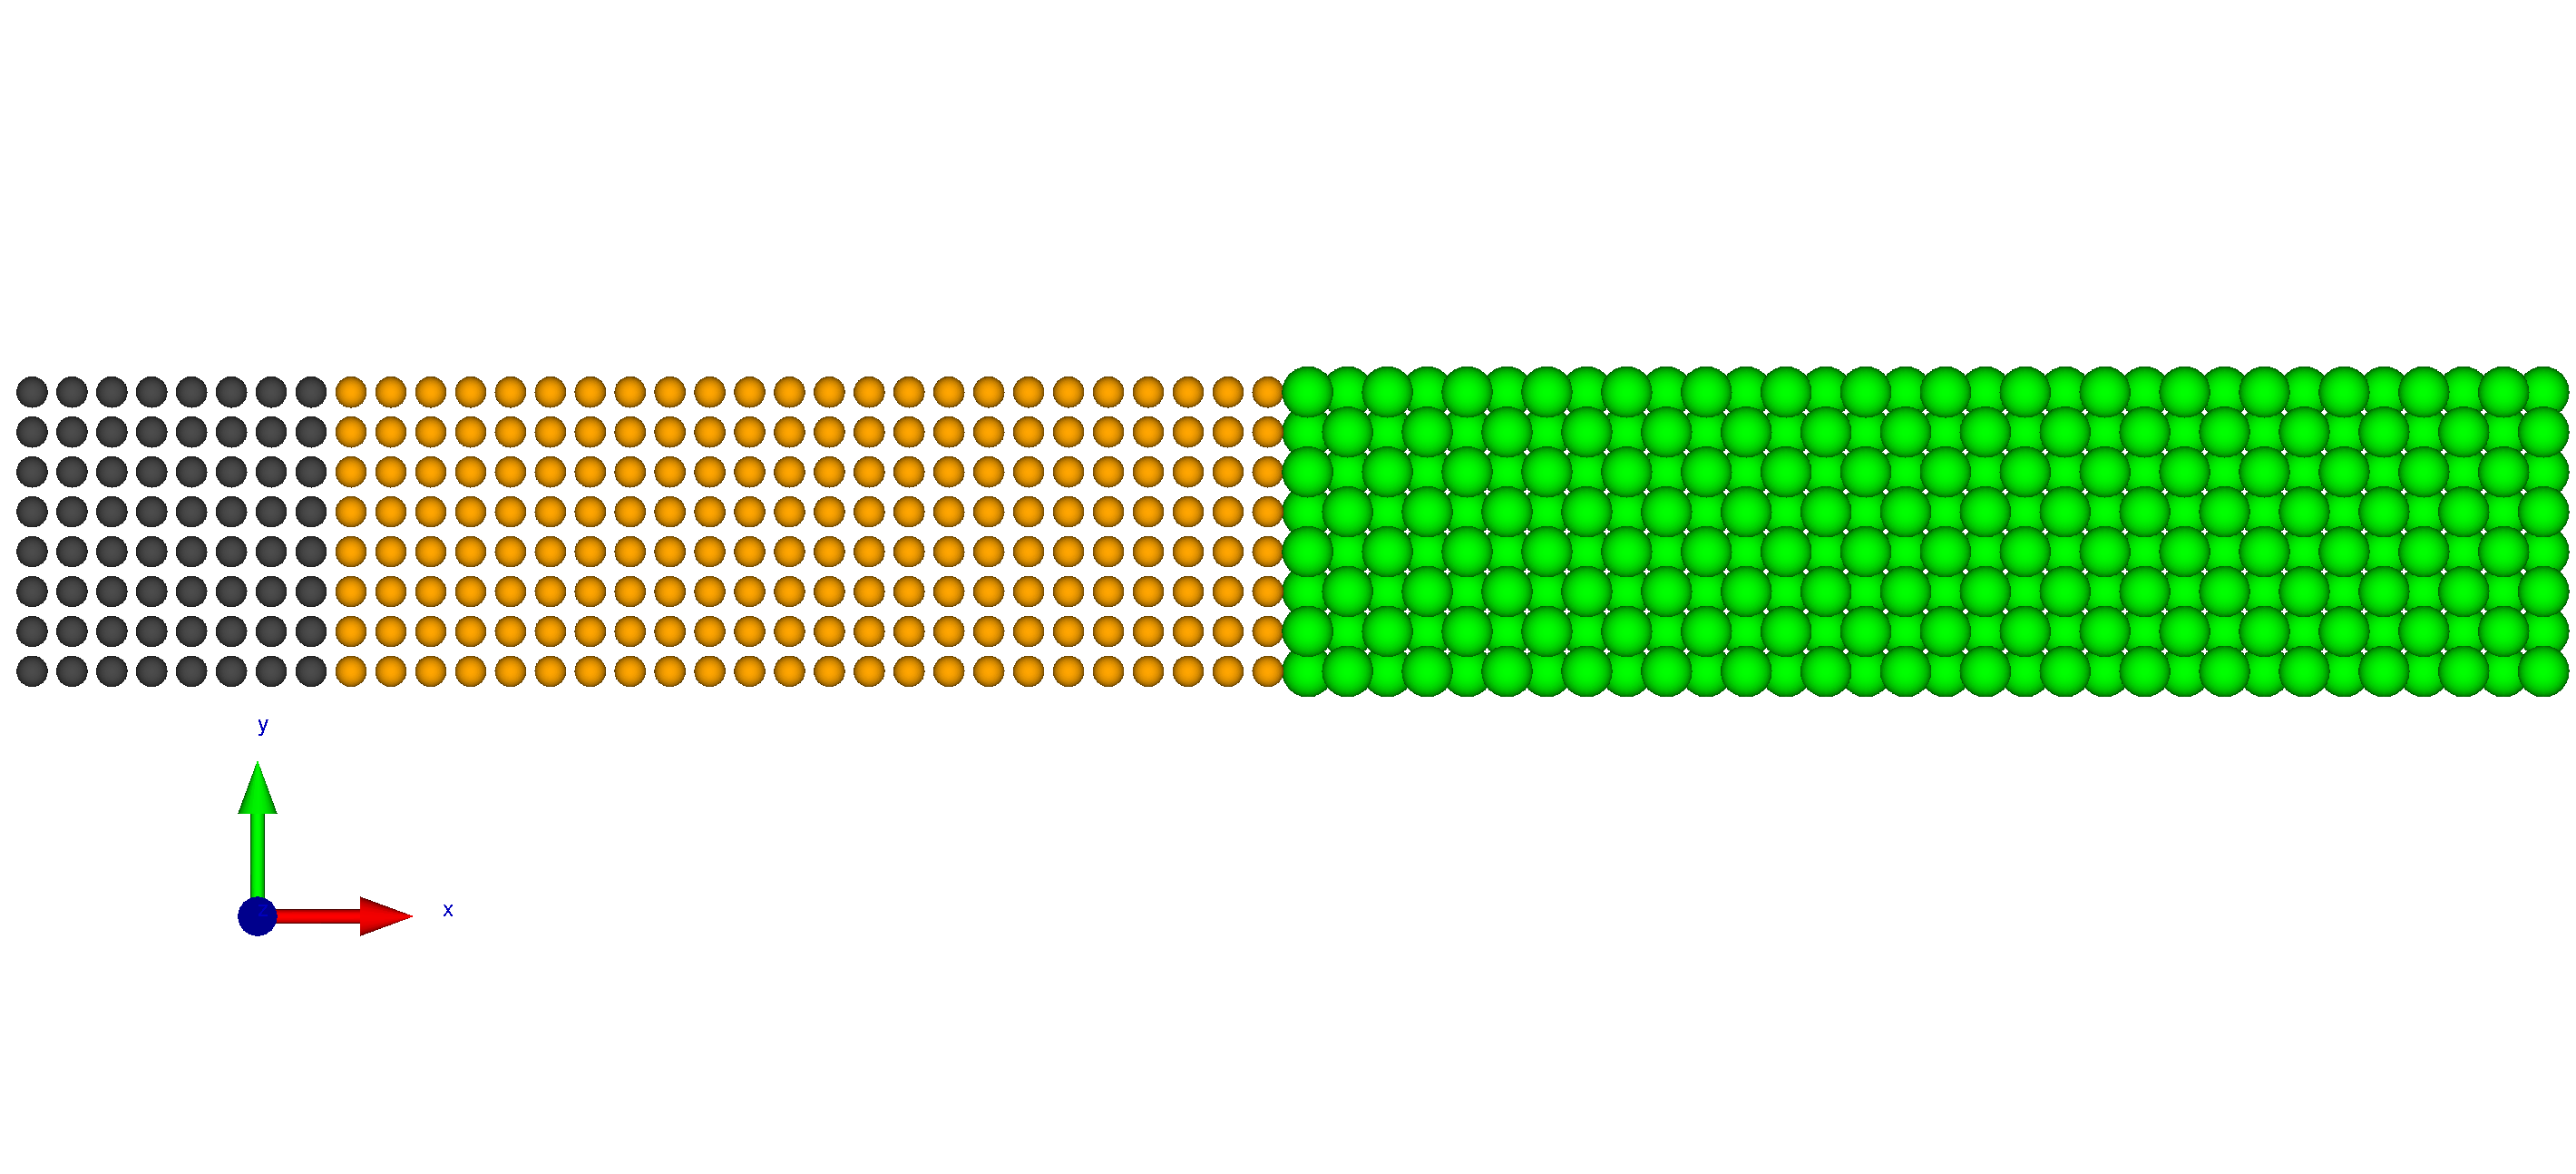
\includegraphics[scale=0.25]{supcell}
\caption{MD domain for interface study of 32x4x4 fcc Argon at 20K with 2048 atoms. Larger atomic radii represents the larger mass.}
\label{fig:subfig1}
\end{figure}
As the plane of the interface has a normal in the $x$ direction, it is reasonable to expect wavevectors containing some $x$ component to be affected. For simplicity, the modes at $\pmb{\kappa}=[1,0,0]$ in the BZ are examined. 
\begin{figure}[h!]
\centering
\subfigure[\small{$\pmb{\kappa}=[1,0,0]$,$\nu=$TA}]{
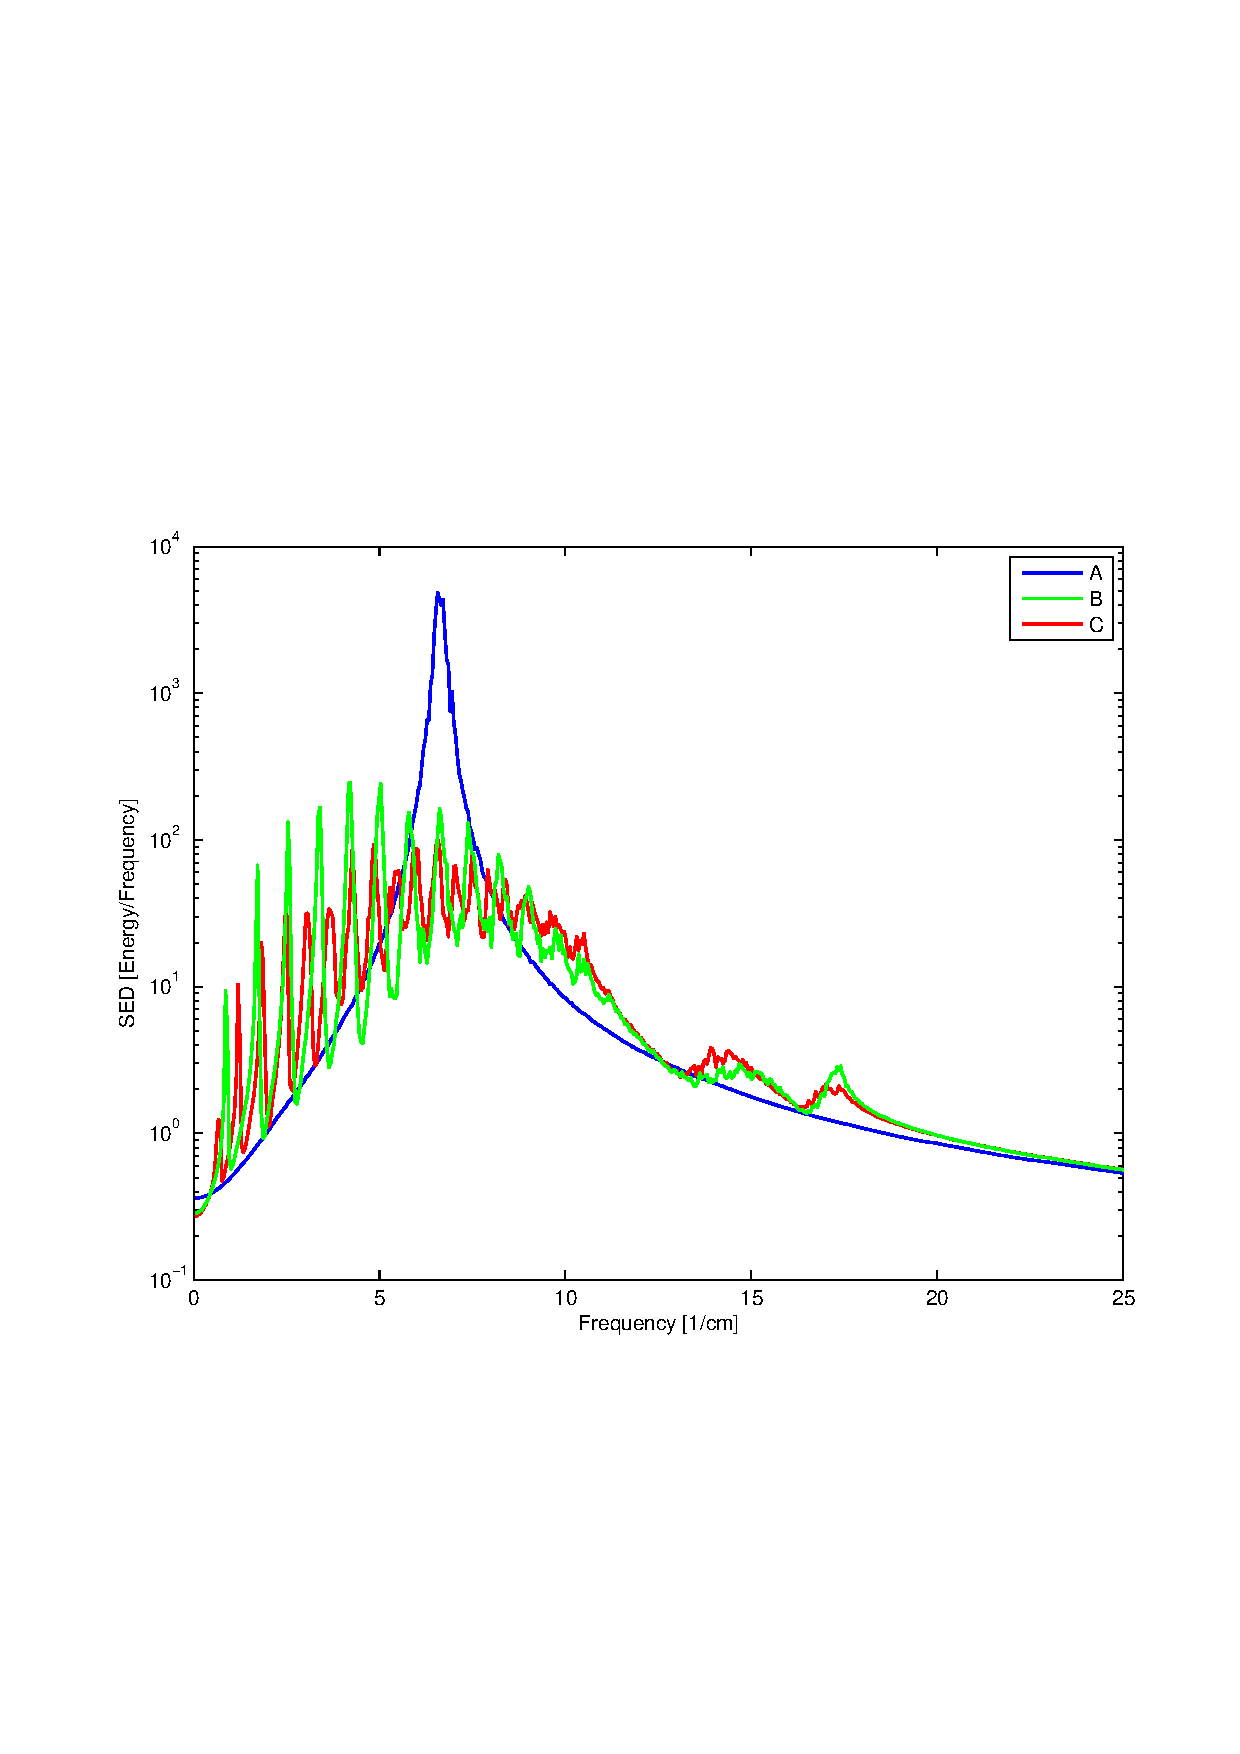
\includegraphics[scale=0.4]{peak_100_TA}
}
\subfigure[\small{$\pmb{\kappa}=[1,0,0]$,$\nu=$LA}]{
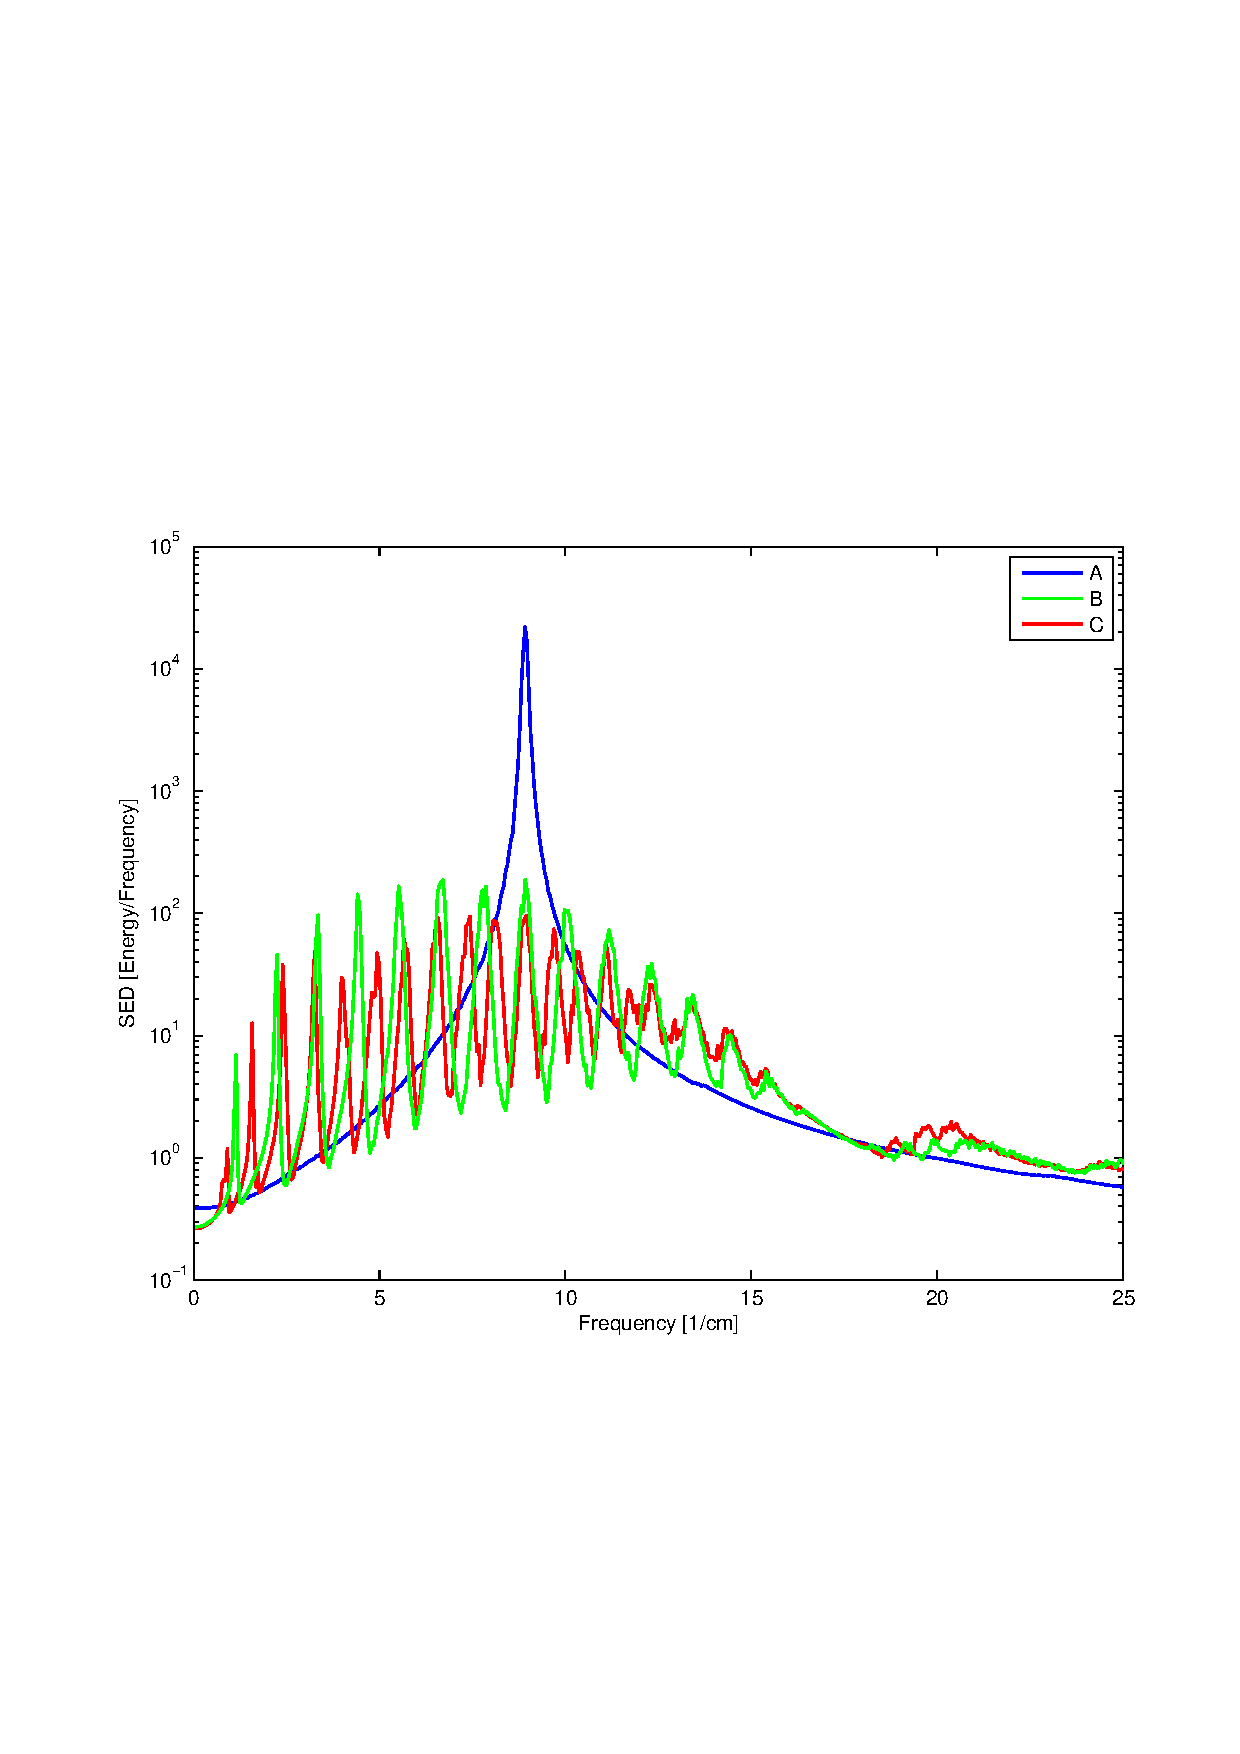
\includegraphics[scale=0.4]{peak_100_LA}
}
\end{figure}
At first glance, it is clear that the SED of Cases B and C differ from Case A. The essence of the difference between Cases B and C and Case A lies not in the physics of the phonons, but in the model of their description. Ultimately, the idea of dividing the 32x4x4 domains into 4x4x4 blocks and performing NMD on these blocks to observe the change in the phonon lifetimes as a function of spatial position relative to the interface proved to be an ineffective approach.

The precise reason for these results is attributed to the mathematical nature of the problem. A sketch of the reason is offered here (a formal argument is presented in the appendix). First, the definition of $Q(\pmb{\kappa},\nu)$ requires the summation over all possible $\pmb{\kappa},\nu$ of the entire 32x4x4 domain. The division into blocks discounts the entire summation to only include available $\pmb{\kappa},\nu$ of the 4x4x4 block:
\begin{eqnarray}
\begin{split}
\dot{Q}(\pmb{\kappa},\nu,t)-\frac{1}{\sqrt{N}}\sum_{28x4x4}\sqrt{m_j}exp(-i\pmb{\kappa}\cdot\pmb{r}(jl))\pmb{e}^*(j,\pmb{\kappa},\nu)\cdot\dot{\pmb{u}}(jl,t)&=\\\frac{1}{\sqrt{N}}\sum_{4x4x4}\sqrt{m_j}exp(-i\pmb{\kappa}\cdot\pmb{r}(jl))\pmb{e}^*(j,\pmb{\kappa},\nu)\cdot\dot{\pmb{u}}(jl,t).
\end{split}
\end{eqnarray}
Neglecting the modes that are uniqe to the complete 32x4x4 domain, leads to an erroneous coordinate transformation from real space to k-space because of the incompleteness of the solution basis. In other words, without using all the possible modes of the system to describe the motion of an individual atom, the corresponding normal mode cannot be inferred. The reverse is equivalently true.

Futhermore, the ensemble of each individual block is difficult to ascertain. The entire domain is fixed to be NVE, but the energy of a block may not be fixed with time (in other words, the Hamiltonian of a block is not time-independent). At any given instant the energy of one block may be more or less than one of its neighbours, but the energy of all the blocks together remains constant.

This exercise revisits the struggle to handle any deviation from the perfectly periodic bulk crystal lattice. By relying on the eigenvectors and frequencies obtained from lattice dynamics, it is not obvious how to incorporate aperiodicities into this approach.

\section*{Future Steps}

The immediate challenge is to try and recover the missing information that is contained in those modes that are present, but discounted from the blocks. This is not trivial. Ultimately, one requires \textit{a priori} knowledge of the time-dependent behaviour of the normal modes. In practice, for a harmonic system, this wouldn't be difficult because the analytical solution of the normal modes is accessible given the initial conditions. For the real anharmonic system, however, this is not an alternative since there is no analytical solution.

A computationally intensive approach would be to perform SED-NMD on the entire domain and use the anharmonic information about the longer wavelength modes to estimate their contribution to these extra SED peaks.

Ostensibly, to investigate this effect requires a fundamentally different view of solids where general aperiodicities, like defects, interfaces, or surfaces can be incorporated. Perhaps the study of phonon properties in amorphous materials will offer insight into this problem.


\newpage
%\bibliographystyle{prb}
\bibliography{new.bib}

\newpage

\section*{Appendix}
\subsection*{Note on the LD eigenvectors}
The difference between Thomas and Larkin's formulation of the SED can be understood through the properties of the eigenvectors. By expanding the kinetic term of the Hamiltonian
\begin{equation}
\begin{split}
\dot{Q}(\pmb{\kappa},\nu)\dot{Q}^*(\pmb{\kappa},\nu)=\frac{1}{N}[\sqrt{m_1}exp(-i\pmb{\kappa}\cdot\pmb{r}(1))\pmb{e}^*(1,\pmb{\kappa},\nu)\cdot\dot{\pmb{u}}(1,t)\\
+\sqrt{m_2}exp(-i\pmb{\kappa}\cdot\pmb{r}(2))\pmb{e}^*(2,\pmb{\kappa},\nu)\cdot\dot{\pmb{u}}(2,t)\\
+...\sqrt{m_n}exp(-i\pmb{\kappa}\cdot\pmb{r}(n))\pmb{e}^*(n,\pmb{\kappa},\nu)\cdot\dot{\pmb{u}}(n,t)\\
+...\sqrt{m_N}exp(-i\pmb{\kappa}\cdot\pmb{r}(N))\pmb{e}^*(N,\pmb{\kappa},\nu)\cdot\dot{\pmb{u}}(N,t)]\\
\times[\sqrt{m_1}exp(i\pmb{\kappa}\cdot\pmb{r}(1))\pmb{e}(1,\pmb{\kappa},\nu)\cdot\dot{\pmb{u}}(1,t)\\
+\sqrt{m_2}exp(i\pmb{\kappa}\cdot\pmb{r}(2))\pmb{e}(2,\pmb{\kappa},\nu)\cdot\dot{\pmb{u}}(2,t)\\
+...\sqrt{m_n}exp(i\pmb{\kappa}\cdot\pmb{r}(n))\pmb{e}(n,\pmb{\kappa},\nu)\cdot\dot{\pmb{u}}(n,t)\\
+...\sqrt{m_N}exp(i\pmb{\kappa}\cdot\pmb{r}(N))\pmb{e}(N,\pmb{\kappa},\nu)\cdot\dot{\pmb{u}}(N,t)]
\end{split}
\end{equation}
From solving the eigenvalue problem of lattice dynamics, the eigenvectors take the form
\[
\pmb{e}(\pmb{\kappa},\nu)=
\begin{pmatrix}
\pmb{e}(1,\pmb{\kappa},\nu)\\
\pmb{e}(2,\pmb{\kappa},\nu)\\
...\\
\pmb{e}(n,\pmb{\kappa},\nu)\\
\end{pmatrix}
\]
where $n$ is the number of atoms in the unit cell and $N$ is the total number of atoms
\begin{equation}
\pmb{e}(1,\pmb{\kappa},\nu)=\pmb{e}(n+1,\pmb{\kappa},\nu)
\end{equation}
\begin{equation}
\pmb{e}(n,\pmb{\kappa},\nu)=\pmb{e}(N,\pmb{\kappa},\nu)
\end{equation}
Recalling that the orthogonality of the eigenvectors ensures 
\begin{equation}
\sum_{j}\pmb{e}(j,\pmb{\kappa},\nu)\cdot\pmb{e}^*(j,\pmb{\kappa},\nu)= \delta_{\pmb{\kappa},\nu:\pmb{\kappa},\nu'}
\end{equation}
\begin{equation}
\pmb{e}(\pmb{\kappa},\nu)\cdot\pmb{e}^*(\pmb{\kappa},\nu)= \delta_{\pmb{\kappa},\nu:\pmb{\kappa},\nu'}
\end{equation}
For the sake of argument, assume this implies
\begin{equation}
\sum_{n'}\pmb{e}(n,\pmb{\kappa},\nu)\cdot\pmb{e}^*(n',\pmb{\kappa},\nu)=\delta_{n:n'}
\end{equation}
If so
\begin{equation}
\dot{Q}(\pmb{\kappa},\nu)\dot{Q}^*(\pmb{\kappa},\nu)=|\frac{1}{\sqrt{N}}\sum_{jl}\sqrt{m_j}\dot{\pmb{u}}(jl,t)|^2
\end{equation}
which is the average kinetic energy of an atom. In theory, the orthogonality applies to the entire eigenvector $\pmb{e}(\pmb{\kappa},\nu)$ but does not imply orthogonality between its components
\begin{equation}
\sum_{n'}\pmb{e}(n,\pmb{\kappa},\nu)\cdot\pmb{e}^*(n',\pmb{\kappa},\nu)\neq\delta_{n:n'}
\end{equation}
It is therefore necessary to project the velocities onto the eigenvectors before calculating the autocorrelation and the SED, since $\dot{Q}(\pmb{\kappa},\nu)\dot{Q}^*(\pmb{\kappa},\nu)$ will have some form resembling the initial expansion in Equation 40.

\subsection*{Insight into the presence of additional peaks}
Consider a linear, nearest neighbour, monotomic chain a with periodic boundary condition, the equations of motions are:
\begin{equation}
\begin{split}
m\ddot{x}_1&=k(x_2-x_1)+k(x_n-x_1)\\
m\ddot{x}_2&=k(x_3-x_2)+k(x_4-x_2)\\
...\\
m\ddot{x}_n&=k(x_{N-1}-x_N)+k(x_1-x_N)\\
\end{split}
\end{equation}
which is a set of coupled linear differential equations. Removing a single equation and the system becomes underdetermined (infinite number of solutions). The matrix version of this system is:
\begin{equation}
\pmb{M}\pmb{\ddot{X}}-\pmb{K}\pmb{X}=0
\end{equation}
With the usual harmonic assumption $\pmb{X}=\pmb{E}e^{i\omega t}$, the problem is recast:
\begin{equation}
[\omega^2\pmb{M}^{-1}\pmb{M}-\pmb{M}^{-1}\pmb{K}]\pmb{E}=0
\end{equation}
Let
\[
\pmb{\psi}=
\begin{bmatrix}
   \pmb{E}_1 & \pmb{E}_2 & \dots &\pmb{E}_n \\
 \end{bmatrix}
\]
We can write $\pmb{\psi}$ as a transformation matrix
\begin{equation}
\begin{split}
\pmb{X}&=\pmb{\psi}\pmb{Q}\\
\pmb{Q}&=\pmb{\psi}^{-1}\pmb{X}
\end{split}
\end{equation}
In relation to the dividing the domain into subdomains, we want to determine $\pmb{Q}$ using a reduced set of $\pmb{X}$, given $\pmb{\psi}$. Looking at a 4 MDOF case, the explicit matrix representation is:
\[
\begin{bmatrix}
   Q_1\\
   Q_2\\
   Q_3\\
   Q_4\\
\end{bmatrix}=
\begin{bmatrix}
   E_{11} & E_{12} & E_{13} & E_{14} \\
   E_{21} & E_{22} & E_{23} & E_{24} \\
   E_{31} & E_{32} & E_{33} & E_{34} \\
   E_{41} & E_{42} & E_{43} & E_{44} \\
\end{bmatrix}^{-1}
\begin{bmatrix}
   x_1\\
   x_2\\
   x_3\\
   x_4\\
\end{bmatrix}
\]
Given a reduced set of $\pmb{X}= [x_1,x_2]$, the equations are rearranged
\begin{equation}
\begin{split}
Q_1-E_{13}'x_3-E_{14}'x_4&= E_{11}'x_1 + E_{12}'x_2\\
Q_2-E_{23}'x_3-E_{24}'x_4&= E_{21}'x_1 + E_{12}'x_2\\
Q_3-E_{33}'x_3-E_{34}'x_4&= E_{31}'x_1 + E_{32}'x_2\\
Q_4-E_{43}'x_3-E_{44}'x_4&= E_{41}'x_1 + E_{42}'x_2.
\end{split}
\end{equation}
This results shows that the transformation from $\pmb{X}$ to $\pmb{Q}$ is relies upon missing information contained with $x_3$ and $x_4$.
\end{document}

